\chapter{Progress To Date}
\label{Chp: Progress To Date}

As a beginning of this project, our first step is to demonstrate that information leakage similar to those described in \cite{Web1} can be found when the underlying protocol is switched DTLS. The reason is that DTLS is more suitable to sensor networks comparing to TLS due to is relatively lightweight-ness. 

The basic idea is to build some toy applications which model typical sensor network traffic generated through DTLS. The information leakage of toy applications are intentionally crafted to emphasise their existence.

Even though both OpenSSL and GnuSSL have DTLS implemented with general features, we setted our experimental the less featured tinyDTLS\cite{tinyDTLS} due to its lightweight-ness, which is more suitable to sensor networks. However, the drawback is that only one cipher-suite, TLS\_ECDHE\_ECDSA\_WITH\_AES\_128\_CCM\_8\cite{rfc7251}, is available for the current version of tinyDTLS. This implies that there should be no padding scheme adopted and hence the length of plaintext and ciphertext are expected to have a linear relationship. Our experiments supported this conjecture such that:
\begin{equation} \label{Eq: Plaintext length}
l_D = 17 + l
\end{equation}
where $l$ is the length of plaintext and $l_D$ is the value in DTLS length field. According to the specifications the additional bytes is supposed to be purely a resulted of the appending MAC even though $17$ bytes is a value unlikely to be. This problem is still under investigating.

All experiments are done with only two processes, a server and a client referred as SERVER and CLIENT, on a same linux host connected through local-link. The protocol suite we adopted is [IPv4 or IPv6] + UDP + DTLS. The modelled adversary is simply a passive eavesdropper.

So far we have built up two toy applications, \textbf{Odd or Even} and \textbf{Leaky Coffee}, which will be explained in the next sessions alongside with corresponding traffic analysis.

\section{Odd or Even} \label{Sec: Odd or Even}
\textbf{Odd or Even} is a simple toy application designed  to demonstrate the fundamental idea of encrypted traffic analysis.

\subsection{Application Description}

\begin{figure}[H] 
\centering
\resizebox{8cm}{!}
{% Graphic for TeX using PGF
% Title: /home/yy12135/MyGit/tinyDTLS-Traffic-Analysis/Writings/First-year-review_20150422/Pics/OddOrEven.dia
% Creator: Dia v0.97.2
% CreationDate: Mon Mar  2 17:12:59 2015
% For: yy12135
% \usepackage{tikz}
% The following commands are not supported in PSTricks at present
% We define them conditionally, so when they are implemented,
% this pgf file will use them.
\ifx\du\undefined
  \newlength{\du}
\fi
\setlength{\du}{15\unitlength}
\begin{tikzpicture}
\pgftransformxscale{1.000000}
\pgftransformyscale{-1.000000}
\definecolor{dialinecolor}{rgb}{0.000000, 0.000000, 0.000000}
\pgfsetstrokecolor{dialinecolor}
\definecolor{dialinecolor}{rgb}{1.000000, 1.000000, 1.000000}
\pgfsetfillcolor{dialinecolor}
% setfont left to latex
\definecolor{dialinecolor}{rgb}{0.000000, 0.000000, 0.000000}
\pgfsetstrokecolor{dialinecolor}
\node[anchor=west] at (11.000000\du,9.000000\du){};
\definecolor{dialinecolor}{rgb}{1.000000, 1.000000, 1.000000}
\pgfsetfillcolor{dialinecolor}
\pgfpathellipse{\pgfpoint{31.003315\du}{10.006491\du}}{\pgfpoint{1.831366\du}{0\du}}{\pgfpoint{0\du}{1.837164\du}}
\pgfusepath{fill}
\pgfsetlinewidth{0.100000\du}
\pgfsetdash{}{0pt}
\pgfsetdash{}{0pt}
\pgfsetmiterjoin
\definecolor{dialinecolor}{rgb}{0.000000, 0.000000, 0.000000}
\pgfsetstrokecolor{dialinecolor}
\pgfpathellipse{\pgfpoint{31.003315\du}{10.006491\du}}{\pgfpoint{1.831366\du}{0\du}}{\pgfpoint{0\du}{1.837164\du}}
\pgfusepath{stroke}
% setfont left to latex
\definecolor{dialinecolor}{rgb}{0.000000, 0.000000, 0.000000}
\pgfsetstrokecolor{dialinecolor}
\node at (31.003315\du,10.201491\du){SERVER};
\pgfsetlinewidth{0.100000\du}
\pgfsetdash{}{0pt}
\pgfsetdash{}{0pt}
\pgfsetbuttcap
{
\definecolor{dialinecolor}{rgb}{0.000000, 0.000000, 0.000000}
\pgfsetfillcolor{dialinecolor}
% was here!!!
\pgfsetarrowsend{stealth}
\definecolor{dialinecolor}{rgb}{0.000000, 0.000000, 0.000000}
\pgfsetstrokecolor{dialinecolor}
\draw (31.002868\du,11.893189\du)--(31.000000\du,24.000000\du);
}
\pgfsetlinewidth{0.100000\du}
\pgfsetdash{}{0pt}
\pgfsetdash{}{0pt}
\pgfsetbuttcap
{
\definecolor{dialinecolor}{rgb}{0.000000, 0.000000, 0.000000}
\pgfsetfillcolor{dialinecolor}
% was here!!!
\pgfsetarrowsend{to}
\definecolor{dialinecolor}{rgb}{0.000000, 0.000000, 0.000000}
\pgfsetstrokecolor{dialinecolor}
\draw (15.036382\du,13.528274\du)--(31.002048\du,15.352278\du);
}
\pgfsetlinewidth{0.100000\du}
\pgfsetdash{}{0pt}
\pgfsetdash{}{0pt}
\pgfsetbuttcap
{
\definecolor{dialinecolor}{rgb}{0.000000, 0.000000, 0.000000}
\pgfsetfillcolor{dialinecolor}
% was here!!!
\pgfsetarrowsend{to}
\definecolor{dialinecolor}{rgb}{0.000000, 0.000000, 0.000000}
\pgfsetstrokecolor{dialinecolor}
\draw (31.001229\du,18.811367\du)--(15.012127\du,20.509425\du);
}
\definecolor{dialinecolor}{rgb}{1.000000, 1.000000, 1.000000}
\pgfsetfillcolor{dialinecolor}
\pgfpathellipse{\pgfpoint{15.048531\du}{10.031365\du}}{\pgfpoint{1.729717\du}{0\du}}{\pgfpoint{0\du}{1.701399\du}}
\pgfusepath{fill}
\pgfsetlinewidth{0.100000\du}
\pgfsetdash{}{0pt}
\pgfsetdash{}{0pt}
\pgfsetmiterjoin
\definecolor{dialinecolor}{rgb}{0.000000, 0.000000, 0.000000}
\pgfsetstrokecolor{dialinecolor}
\pgfpathellipse{\pgfpoint{15.048531\du}{10.031365\du}}{\pgfpoint{1.729717\du}{0\du}}{\pgfpoint{0\du}{1.701399\du}}
\pgfusepath{stroke}
% setfont left to latex
\definecolor{dialinecolor}{rgb}{0.000000, 0.000000, 0.000000}
\pgfsetstrokecolor{dialinecolor}
\node at (15.048531\du,10.226365\du){CLIENT};
\pgfsetlinewidth{0.100000\du}
\pgfsetdash{}{0pt}
\pgfsetdash{}{0pt}
\pgfsetbuttcap
{
\definecolor{dialinecolor}{rgb}{0.000000, 0.000000, 0.000000}
\pgfsetfillcolor{dialinecolor}
% was here!!!
\pgfsetarrowsend{stealth}
\definecolor{dialinecolor}{rgb}{0.000000, 0.000000, 0.000000}
\pgfsetstrokecolor{dialinecolor}
\draw (15.042445\du,11.782986\du)--(15.000000\du,24.000000\du);
}
\pgfsetlinewidth{0.100000\du}
\pgfsetdash{}{0pt}
\pgfsetdash{}{0pt}
\pgfsetbuttcap
\pgfsetmiterjoin
\pgfsetlinewidth{0.100000\du}
\pgfsetbuttcap
\pgfsetmiterjoin
\pgfsetdash{}{0pt}
\definecolor{dialinecolor}{rgb}{1.000000, 1.000000, 1.000000}
\pgfsetfillcolor{dialinecolor}
\pgfpathmoveto{\pgfpoint{20.833333\du}{13.000000\du}}
\pgfpathlineto{\pgfpoint{24.166667\du}{13.000000\du}}
\pgfpathcurveto{\pgfpoint{24.626904\du}{13.000000\du}}{\pgfpoint{25.000000\du}{13.447715\du}}{\pgfpoint{25.000000\du}{14.000000\du}}
\pgfpathcurveto{\pgfpoint{25.000000\du}{14.552285\du}}{\pgfpoint{24.626904\du}{15.000000\du}}{\pgfpoint{24.166667\du}{15.000000\du}}
\pgfpathlineto{\pgfpoint{20.833333\du}{15.000000\du}}
\pgfpathcurveto{\pgfpoint{20.373096\du}{15.000000\du}}{\pgfpoint{20.000000\du}{14.552285\du}}{\pgfpoint{20.000000\du}{14.000000\du}}
\pgfpathcurveto{\pgfpoint{20.000000\du}{13.447715\du}}{\pgfpoint{20.373096\du}{13.000000\du}}{\pgfpoint{20.833333\du}{13.000000\du}}
\pgfusepath{fill}
\definecolor{dialinecolor}{rgb}{0.000000, 0.000000, 0.000000}
\pgfsetstrokecolor{dialinecolor}
\pgfpathmoveto{\pgfpoint{20.833333\du}{13.000000\du}}
\pgfpathlineto{\pgfpoint{24.166667\du}{13.000000\du}}
\pgfpathcurveto{\pgfpoint{24.626904\du}{13.000000\du}}{\pgfpoint{25.000000\du}{13.447715\du}}{\pgfpoint{25.000000\du}{14.000000\du}}
\pgfpathcurveto{\pgfpoint{25.000000\du}{14.552285\du}}{\pgfpoint{24.626904\du}{15.000000\du}}{\pgfpoint{24.166667\du}{15.000000\du}}
\pgfpathlineto{\pgfpoint{20.833333\du}{15.000000\du}}
\pgfpathcurveto{\pgfpoint{20.373096\du}{15.000000\du}}{\pgfpoint{20.000000\du}{14.552285\du}}{\pgfpoint{20.000000\du}{14.000000\du}}
\pgfpathcurveto{\pgfpoint{20.000000\du}{13.447715\du}}{\pgfpoint{20.373096\du}{13.000000\du}}{\pgfpoint{20.833333\du}{13.000000\du}}
\pgfusepath{stroke}
% setfont left to latex
\definecolor{dialinecolor}{rgb}{0.000000, 0.000000, 0.000000}
\pgfsetstrokecolor{dialinecolor}
\node at (22.500000\du,14.200000\du){32bit R};
\pgfsetlinewidth{0.100000\du}
\pgfsetdash{}{0pt}
\pgfsetdash{}{0pt}
\pgfsetbuttcap
\pgfsetmiterjoin
\pgfsetlinewidth{0.100000\du}
\pgfsetbuttcap
\pgfsetmiterjoin
\pgfsetdash{}{0pt}
\definecolor{dialinecolor}{rgb}{1.000000, 1.000000, 1.000000}
\pgfsetfillcolor{dialinecolor}
\pgfpathmoveto{\pgfpoint{20.228125\du}{18.000000\du}}
\pgfpathlineto{\pgfpoint{25.140625\du}{18.000000\du}}
\pgfpathcurveto{\pgfpoint{25.818900\du}{18.000000\du}}{\pgfpoint{26.368750\du}{18.447715\du}}{\pgfpoint{26.368750\du}{19.000000\du}}
\pgfpathcurveto{\pgfpoint{26.368750\du}{19.552285\du}}{\pgfpoint{25.818900\du}{20.000000\du}}{\pgfpoint{25.140625\du}{20.000000\du}}
\pgfpathlineto{\pgfpoint{20.228125\du}{20.000000\du}}
\pgfpathcurveto{\pgfpoint{19.549850\du}{20.000000\du}}{\pgfpoint{19.000000\du}{19.552285\du}}{\pgfpoint{19.000000\du}{19.000000\du}}
\pgfpathcurveto{\pgfpoint{19.000000\du}{18.447715\du}}{\pgfpoint{19.549850\du}{18.000000\du}}{\pgfpoint{20.228125\du}{18.000000\du}}
\pgfusepath{fill}
\definecolor{dialinecolor}{rgb}{0.000000, 0.000000, 0.000000}
\pgfsetstrokecolor{dialinecolor}
\pgfpathmoveto{\pgfpoint{20.228125\du}{18.000000\du}}
\pgfpathlineto{\pgfpoint{25.140625\du}{18.000000\du}}
\pgfpathcurveto{\pgfpoint{25.818900\du}{18.000000\du}}{\pgfpoint{26.368750\du}{18.447715\du}}{\pgfpoint{26.368750\du}{19.000000\du}}
\pgfpathcurveto{\pgfpoint{26.368750\du}{19.552285\du}}{\pgfpoint{25.818900\du}{20.000000\du}}{\pgfpoint{25.140625\du}{20.000000\du}}
\pgfpathlineto{\pgfpoint{20.228125\du}{20.000000\du}}
\pgfpathcurveto{\pgfpoint{19.549850\du}{20.000000\du}}{\pgfpoint{19.000000\du}{19.552285\du}}{\pgfpoint{19.000000\du}{19.000000\du}}
\pgfpathcurveto{\pgfpoint{19.000000\du}{18.447715\du}}{\pgfpoint{19.549850\du}{18.000000\du}}{\pgfpoint{20.228125\du}{18.000000\du}}
\pgfusepath{stroke}
% setfont left to latex
\definecolor{dialinecolor}{rgb}{0.000000, 0.000000, 0.000000}
\pgfsetstrokecolor{dialinecolor}
\node at (22.684375\du,19.200000\du){"ODD"/"EVEN"};
\end{tikzpicture}
}
\caption{Description of an Odd-or-Even session}
\label{Fig: Odd or Even}
\end{figure}

CLIENT randomly generates a 32-bit unsigned integer R and sends it to SERVER in binary. SERVER replies with a string “ODD'' or “EVEN” according to the value of the 32-bit $R$(\Cref{Fig: Odd or Even}).

\subsection{Analysis}
We run the application for multiple times and collected the packets it generated. As we have expected, “ODD” packets are $1$ byte shorter than “EVEN” packets which implies that an eavesdropping adversary can learn what has been sent from SERVER to CLIENT simply by looking at the packets length. However, no obvious leakage has been found in other fields of the packets.

%For every \textbf{Odd-or-Even} session, 
%
%Packets from CLIENT to SERVER:
%
%All fields for every packet are the same, except:
%1. Encrypted Application Data field in DTLS layer.
%2. Sequence Number increased by 1 every packet.
%3. Checksum in UDP layer.
%
%Packets from SERVER to CLIENT:
%
%All fields are the same for every packet except:
%1. Encrypted Application Data field in DTLS layer.
%2. Sequence Number increased by 1 every packet.
%3. Checksum in UDP layer.
%4. Length field in both DTLS layer and UDP layer. The values are always (20,41) respectively when data is "Odd" and (21,42) when data is "Even".
%
%Therefore in this application, given pre-knowledge that server responds with either "Odd" or "Even", the length field in both DTLS layer and UDP layer can directly leak the plaintext. 

\section{Leaky Coffee}
\label{Sec: Leaky Coffee}

\subsection{Application Description}
\textbf{Leaky Coffee} simulates a more complicated scenario where the CLIENT sends a coffee order (in string) to SERVER. SERVER echoes the order appended by some flavour (in string). CLIENT compares the amount of given flavour to an internally generated random requirement and asks SERVER again for more additive if it is insufficient.

\begin{figure}[H]
\centering
\resizebox{12cm}{!}
{% Graphic for TeX using PGF
% Title: /home/yy12135/Google Drive/Writings/First-year-review_20150422/Pics/LeakyCoffee.dia
% Creator: Dia v0.97.2
% CreationDate: Tue Mar  3 14:05:39 2015
% For: yy12135
% \usepackage{tikz}
% The following commands are not supported in PSTricks at present
% We define them conditionally, so when they are implemented,
% this pgf file will use them.
\ifx\du\undefined
  \newlength{\du}
\fi
\setlength{\du}{15\unitlength}
\begin{tikzpicture}
\pgftransformxscale{1.000000}
\pgftransformyscale{-1.000000}
\definecolor{dialinecolor}{rgb}{0.000000, 0.000000, 0.000000}
\pgfsetstrokecolor{dialinecolor}
\definecolor{dialinecolor}{rgb}{1.000000, 1.000000, 1.000000}
\pgfsetfillcolor{dialinecolor}
\definecolor{dialinecolor}{rgb}{1.000000, 1.000000, 1.000000}
\pgfsetfillcolor{dialinecolor}
\pgfpathellipse{\pgfpoint{10.000000\du}{11.000000\du}}{\pgfpoint{1.723870\du}{0\du}}{\pgfpoint{0\du}{1.723870\du}}
\pgfusepath{fill}
\pgfsetlinewidth{0.100000\du}
\pgfsetdash{}{0pt}
\pgfsetdash{}{0pt}
\pgfsetmiterjoin
\definecolor{dialinecolor}{rgb}{0.000000, 0.000000, 0.000000}
\pgfsetstrokecolor{dialinecolor}
\pgfpathellipse{\pgfpoint{10.000000\du}{11.000000\du}}{\pgfpoint{1.723870\du}{0\du}}{\pgfpoint{0\du}{1.723870\du}}
\pgfusepath{stroke}
% setfont left to latex
\definecolor{dialinecolor}{rgb}{0.000000, 0.000000, 0.000000}
\pgfsetstrokecolor{dialinecolor}
\node at (10.000000\du,11.195000\du){CLIENT};
% setfont left to latex
\definecolor{dialinecolor}{rgb}{0.000000, 0.000000, 0.000000}
\pgfsetstrokecolor{dialinecolor}
\node[anchor=west] at (10.000000\du,11.000000\du){};
\definecolor{dialinecolor}{rgb}{1.000000, 1.000000, 1.000000}
\pgfsetfillcolor{dialinecolor}
\pgfpathellipse{\pgfpoint{25.008494\du}{10.996126\du}}{\pgfpoint{1.836494\du}{0\du}}{\pgfpoint{0\du}{1.813886\du}}
\pgfusepath{fill}
\pgfsetlinewidth{0.100000\du}
\pgfsetdash{}{0pt}
\pgfsetdash{}{0pt}
\pgfsetmiterjoin
\definecolor{dialinecolor}{rgb}{0.000000, 0.000000, 0.000000}
\pgfsetstrokecolor{dialinecolor}
\pgfpathellipse{\pgfpoint{25.008494\du}{10.996126\du}}{\pgfpoint{1.836494\du}{0\du}}{\pgfpoint{0\du}{1.813886\du}}
\pgfusepath{stroke}
% setfont left to latex
\definecolor{dialinecolor}{rgb}{0.000000, 0.000000, 0.000000}
\pgfsetstrokecolor{dialinecolor}
\node at (25.008494\du,11.191126\du){SERVER};
\pgfsetlinewidth{0.100000\du}
\pgfsetdash{}{0pt}
\pgfsetdash{}{0pt}
\pgfsetbuttcap
{
\definecolor{dialinecolor}{rgb}{0.000000, 0.000000, 0.000000}
\pgfsetfillcolor{dialinecolor}
% was here!!!
\pgfsetarrowsend{to}
\definecolor{dialinecolor}{rgb}{0.000000, 0.000000, 0.000000}
\pgfsetstrokecolor{dialinecolor}
\draw (10.000000\du,12.774002\du)--(10.000000\du,40.000000\du);
}
\pgfsetlinewidth{0.100000\du}
\pgfsetdash{}{0pt}
\pgfsetdash{}{0pt}
\pgfsetbuttcap
{
\definecolor{dialinecolor}{rgb}{0.000000, 0.000000, 0.000000}
\pgfsetfillcolor{dialinecolor}
% was here!!!
\pgfsetarrowsend{to}
\definecolor{dialinecolor}{rgb}{0.000000, 0.000000, 0.000000}
\pgfsetstrokecolor{dialinecolor}
\draw (25.007949\du,12.859321\du)--(25.000000\du,40.000000\du);
}
\pgfsetlinewidth{0.100000\du}
\pgfsetdash{}{0pt}
\pgfsetdash{}{0pt}
\pgfsetbuttcap
{
\definecolor{dialinecolor}{rgb}{0.000000, 0.000000, 0.000000}
\pgfsetfillcolor{dialinecolor}
% was here!!!
\pgfsetarrowsend{to}
\definecolor{dialinecolor}{rgb}{0.000000, 0.000000, 0.000000}
\pgfsetstrokecolor{dialinecolor}
\draw (10.000000\du,15.799100\du)--(25.006200\du,18.890600\du);
}
\pgfsetlinewidth{0.100000\du}
\pgfsetdash{}{0pt}
\pgfsetdash{}{0pt}
\pgfsetbuttcap
{
\definecolor{dialinecolor}{rgb}{0.000000, 0.000000, 0.000000}
\pgfsetfillcolor{dialinecolor}
% was here!!!
\pgfsetarrowsend{to}
\definecolor{dialinecolor}{rgb}{0.000000, 0.000000, 0.000000}
\pgfsetstrokecolor{dialinecolor}
\draw (25.005300\du,21.906200\du)--(10.000000\du,24.874400\du);
}
\pgfsetlinewidth{0.100000\du}
\pgfsetdash{}{0pt}
\pgfsetdash{}{0pt}
\pgfsetbuttcap
\pgfsetmiterjoin
\pgfsetlinewidth{0.100000\du}
\pgfsetbuttcap
\pgfsetmiterjoin
\pgfsetdash{}{0pt}
\definecolor{dialinecolor}{rgb}{1.000000, 1.000000, 1.000000}
\pgfsetfillcolor{dialinecolor}
\pgfpathmoveto{\pgfpoint{13.558175\du}{16.000000\du}}
\pgfpathlineto{\pgfpoint{19.625675\du}{16.000000\du}}
\pgfpathcurveto{\pgfpoint{20.463422\du}{16.000000\du}}{\pgfpoint{21.142550\du}{16.447715\du}}{\pgfpoint{21.142550\du}{17.000000\du}}
\pgfpathcurveto{\pgfpoint{21.142550\du}{17.552285\du}}{\pgfpoint{20.463422\du}{18.000000\du}}{\pgfpoint{19.625675\du}{18.000000\du}}
\pgfpathlineto{\pgfpoint{13.558175\du}{18.000000\du}}
\pgfpathcurveto{\pgfpoint{12.720428\du}{18.000000\du}}{\pgfpoint{12.041300\du}{17.552285\du}}{\pgfpoint{12.041300\du}{17.000000\du}}
\pgfpathcurveto{\pgfpoint{12.041300\du}{16.447715\du}}{\pgfpoint{12.720428\du}{16.000000\du}}{\pgfpoint{13.558175\du}{16.000000\du}}
\pgfusepath{fill}
\definecolor{dialinecolor}{rgb}{0.000000, 0.000000, 0.000000}
\pgfsetstrokecolor{dialinecolor}
\pgfpathmoveto{\pgfpoint{13.558175\du}{16.000000\du}}
\pgfpathlineto{\pgfpoint{19.625675\du}{16.000000\du}}
\pgfpathcurveto{\pgfpoint{20.463422\du}{16.000000\du}}{\pgfpoint{21.142550\du}{16.447715\du}}{\pgfpoint{21.142550\du}{17.000000\du}}
\pgfpathcurveto{\pgfpoint{21.142550\du}{17.552285\du}}{\pgfpoint{20.463422\du}{18.000000\du}}{\pgfpoint{19.625675\du}{18.000000\du}}
\pgfpathlineto{\pgfpoint{13.558175\du}{18.000000\du}}
\pgfpathcurveto{\pgfpoint{12.720428\du}{18.000000\du}}{\pgfpoint{12.041300\du}{17.552285\du}}{\pgfpoint{12.041300\du}{17.000000\du}}
\pgfpathcurveto{\pgfpoint{12.041300\du}{16.447715\du}}{\pgfpoint{12.720428\du}{16.000000\du}}{\pgfpoint{13.558175\du}{16.000000\du}}
\pgfusepath{stroke}
% setfont left to latex
\definecolor{dialinecolor}{rgb}{0.000000, 0.000000, 0.000000}
\pgfsetstrokecolor{dialinecolor}
\node at (16.591925\du,17.200000\du){\textbf{1}. $Order$};
\pgfsetlinewidth{0.100000\du}
\pgfsetdash{}{0pt}
\pgfsetdash{}{0pt}
\pgfsetbuttcap
\pgfsetmiterjoin
\pgfsetlinewidth{0.100000\du}
\pgfsetbuttcap
\pgfsetmiterjoin
\pgfsetdash{}{0pt}
\definecolor{dialinecolor}{rgb}{1.000000, 1.000000, 1.000000}
\pgfsetfillcolor{dialinecolor}
\pgfpathmoveto{\pgfpoint{12.990000\du}{22.000000\du}}
\pgfpathlineto{\pgfpoint{20.950000\du}{22.000000\du}}
\pgfpathcurveto{\pgfpoint{22.049047\du}{22.000000\du}}{\pgfpoint{22.940000\du}{22.447715\du}}{\pgfpoint{22.940000\du}{23.000000\du}}
\pgfpathcurveto{\pgfpoint{22.940000\du}{23.552285\du}}{\pgfpoint{22.049047\du}{24.000000\du}}{\pgfpoint{20.950000\du}{24.000000\du}}
\pgfpathlineto{\pgfpoint{12.990000\du}{24.000000\du}}
\pgfpathcurveto{\pgfpoint{11.890953\du}{24.000000\du}}{\pgfpoint{11.000000\du}{23.552285\du}}{\pgfpoint{11.000000\du}{23.000000\du}}
\pgfpathcurveto{\pgfpoint{11.000000\du}{22.447715\du}}{\pgfpoint{11.890953\du}{22.000000\du}}{\pgfpoint{12.990000\du}{22.000000\du}}
\pgfusepath{fill}
\definecolor{dialinecolor}{rgb}{0.000000, 0.000000, 0.000000}
\pgfsetstrokecolor{dialinecolor}
\pgfpathmoveto{\pgfpoint{12.990000\du}{22.000000\du}}
\pgfpathlineto{\pgfpoint{20.950000\du}{22.000000\du}}
\pgfpathcurveto{\pgfpoint{22.049047\du}{22.000000\du}}{\pgfpoint{22.940000\du}{22.447715\du}}{\pgfpoint{22.940000\du}{23.000000\du}}
\pgfpathcurveto{\pgfpoint{22.940000\du}{23.552285\du}}{\pgfpoint{22.049047\du}{24.000000\du}}{\pgfpoint{20.950000\du}{24.000000\du}}
\pgfpathlineto{\pgfpoint{12.990000\du}{24.000000\du}}
\pgfpathcurveto{\pgfpoint{11.890953\du}{24.000000\du}}{\pgfpoint{11.000000\du}{23.552285\du}}{\pgfpoint{11.000000\du}{23.000000\du}}
\pgfpathcurveto{\pgfpoint{11.000000\du}{22.447715\du}}{\pgfpoint{11.890953\du}{22.000000\du}}{\pgfpoint{12.990000\du}{22.000000\du}}
\pgfusepath{stroke}
% setfont left to latex
\definecolor{dialinecolor}{rgb}{0.000000, 0.000000, 0.000000}
\pgfsetstrokecolor{dialinecolor}
\node at (16.970000\du,23.200000\du){\textbf{2}.$Coffee$};
\pgfsetlinewidth{0.100000\du}
\pgfsetdash{{1.000000\du}{1.000000\du}}{0\du}
\pgfsetdash{{1.000000\du}{1.000000\du}}{0\du}
\pgfsetbuttcap
{
\definecolor{dialinecolor}{rgb}{0.000000, 0.000000, 0.000000}
\pgfsetfillcolor{dialinecolor}
% was here!!!
\definecolor{dialinecolor}{rgb}{0.000000, 0.000000, 0.000000}
\pgfsetstrokecolor{dialinecolor}
\draw (9.010000\du,25.950000\du)--(36.000000\du,26.000000\du);
}
\definecolor{dialinecolor}{rgb}{1.000000, 1.000000, 1.000000}
\pgfsetfillcolor{dialinecolor}
\fill (0.000000\du,25.000000\du)--(0.000000\du,26.900000\du)--(9.010000\du,26.900000\du)--(9.010000\du,25.000000\du)--cycle;
\pgfsetlinewidth{0.100000\du}
\pgfsetdash{}{0pt}
\pgfsetdash{}{0pt}
\pgfsetmiterjoin
\definecolor{dialinecolor}{rgb}{0.000000, 0.000000, 0.000000}
\pgfsetstrokecolor{dialinecolor}
\draw (0.000000\du,25.000000\du)--(0.000000\du,26.900000\du)--(9.010000\du,26.900000\du)--(9.010000\du,25.000000\du)--cycle;
% setfont left to latex
\definecolor{dialinecolor}{rgb}{0.000000, 0.000000, 0.000000}
\pgfsetstrokecolor{dialinecolor}
\node at (4.505000\du,26.145000\du){If $Flavour$ is not enough};
\pgfsetlinewidth{0.100000\du}
\pgfsetdash{}{0pt}
\pgfsetdash{}{0pt}
\pgfsetbuttcap
{
\definecolor{dialinecolor}{rgb}{0.000000, 0.000000, 0.000000}
\pgfsetfillcolor{dialinecolor}
% was here!!!
\pgfsetarrowsend{to}
\definecolor{dialinecolor}{rgb}{0.000000, 0.000000, 0.000000}
\pgfsetstrokecolor{dialinecolor}
\draw (10.000000\du,27.899600\du)--(25.002700\du,30.953100\du);
}
\pgfsetlinewidth{0.100000\du}
\pgfsetdash{}{0pt}
\pgfsetdash{}{0pt}
\pgfsetbuttcap
\pgfsetmiterjoin
\pgfsetlinewidth{0.100000\du}
\pgfsetbuttcap
\pgfsetmiterjoin
\pgfsetdash{}{0pt}
\definecolor{dialinecolor}{rgb}{1.000000, 1.000000, 1.000000}
\pgfsetfillcolor{dialinecolor}
\pgfpathmoveto{\pgfpoint{14.065625\du}{28.000000\du}}
\pgfpathlineto{\pgfpoint{20.158125\du}{28.000000\du}}
\pgfpathcurveto{\pgfpoint{20.999324\du}{28.000000\du}}{\pgfpoint{21.681250\du}{28.447715\du}}{\pgfpoint{21.681250\du}{29.000000\du}}
\pgfpathcurveto{\pgfpoint{21.681250\du}{29.552285\du}}{\pgfpoint{20.999324\du}{30.000000\du}}{\pgfpoint{20.158125\du}{30.000000\du}}
\pgfpathlineto{\pgfpoint{14.065625\du}{30.000000\du}}
\pgfpathcurveto{\pgfpoint{13.224426\du}{30.000000\du}}{\pgfpoint{12.542500\du}{29.552285\du}}{\pgfpoint{12.542500\du}{29.000000\du}}
\pgfpathcurveto{\pgfpoint{12.542500\du}{28.447715\du}}{\pgfpoint{13.224426\du}{28.000000\du}}{\pgfpoint{14.065625\du}{28.000000\du}}
\pgfusepath{fill}
\definecolor{dialinecolor}{rgb}{0.000000, 0.000000, 0.000000}
\pgfsetstrokecolor{dialinecolor}
\pgfpathmoveto{\pgfpoint{14.065625\du}{28.000000\du}}
\pgfpathlineto{\pgfpoint{20.158125\du}{28.000000\du}}
\pgfpathcurveto{\pgfpoint{20.999324\du}{28.000000\du}}{\pgfpoint{21.681250\du}{28.447715\du}}{\pgfpoint{21.681250\du}{29.000000\du}}
\pgfpathcurveto{\pgfpoint{21.681250\du}{29.552285\du}}{\pgfpoint{20.999324\du}{30.000000\du}}{\pgfpoint{20.158125\du}{30.000000\du}}
\pgfpathlineto{\pgfpoint{14.065625\du}{30.000000\du}}
\pgfpathcurveto{\pgfpoint{13.224426\du}{30.000000\du}}{\pgfpoint{12.542500\du}{29.552285\du}}{\pgfpoint{12.542500\du}{29.000000\du}}
\pgfpathcurveto{\pgfpoint{12.542500\du}{28.447715\du}}{\pgfpoint{13.224426\du}{28.000000\du}}{\pgfpoint{14.065625\du}{28.000000\du}}
\pgfusepath{stroke}
% setfont left to latex
\definecolor{dialinecolor}{rgb}{0.000000, 0.000000, 0.000000}
\pgfsetstrokecolor{dialinecolor}
\node at (17.111875\du,29.200000\du){\textbf{3}.$FlavourRequest$};
\pgfsetlinewidth{0.100000\du}
\pgfsetdash{{1.000000\du}{1.000000\du}}{0\du}
\pgfsetdash{{1.000000\du}{1.000000\du}}{0\du}
\pgfsetbuttcap
{
\definecolor{dialinecolor}{rgb}{0.000000, 0.000000, 0.000000}
\pgfsetfillcolor{dialinecolor}
% was here!!!
\definecolor{dialinecolor}{rgb}{0.000000, 0.000000, 0.000000}
\pgfsetstrokecolor{dialinecolor}
\draw (1.000000\du,38.000000\du)--(36.000000\du,38.000000\du);
}
\pgfsetlinewidth{0.100000\du}
\pgfsetdash{}{0pt}
\pgfsetdash{}{0pt}
\pgfsetbuttcap
{
\definecolor{dialinecolor}{rgb}{0.000000, 0.000000, 0.000000}
\pgfsetfillcolor{dialinecolor}
% was here!!!
\pgfsetarrowsend{to}
\definecolor{dialinecolor}{rgb}{0.000000, 0.000000, 0.000000}
\pgfsetstrokecolor{dialinecolor}
\draw (25.001800\du,33.968700\du)--(10.000000\du,36.974900\du);
}
\pgfsetlinewidth{0.100000\du}
\pgfsetdash{}{0pt}
\pgfsetdash{}{0pt}
\pgfsetbuttcap
\pgfsetmiterjoin
\pgfsetlinewidth{0.100000\du}
\pgfsetbuttcap
\pgfsetmiterjoin
\pgfsetdash{}{0pt}
\definecolor{dialinecolor}{rgb}{1.000000, 1.000000, 1.000000}
\pgfsetfillcolor{dialinecolor}
\pgfpathmoveto{\pgfpoint{13.779375\du}{34.000000\du}}
\pgfpathlineto{\pgfpoint{20.236875\du}{34.000000\du}}
\pgfpathcurveto{\pgfpoint{21.128470\du}{34.000000\du}}{\pgfpoint{21.851250\du}{34.447715\du}}{\pgfpoint{21.851250\du}{35.000000\du}}
\pgfpathcurveto{\pgfpoint{21.851250\du}{35.552285\du}}{\pgfpoint{21.128470\du}{36.000000\du}}{\pgfpoint{20.236875\du}{36.000000\du}}
\pgfpathlineto{\pgfpoint{13.779375\du}{36.000000\du}}
\pgfpathcurveto{\pgfpoint{12.887780\du}{36.000000\du}}{\pgfpoint{12.165000\du}{35.552285\du}}{\pgfpoint{12.165000\du}{35.000000\du}}
\pgfpathcurveto{\pgfpoint{12.165000\du}{34.447715\du}}{\pgfpoint{12.887780\du}{34.000000\du}}{\pgfpoint{13.779375\du}{34.000000\du}}
\pgfusepath{fill}
\definecolor{dialinecolor}{rgb}{0.000000, 0.000000, 0.000000}
\pgfsetstrokecolor{dialinecolor}
\pgfpathmoveto{\pgfpoint{13.779375\du}{34.000000\du}}
\pgfpathlineto{\pgfpoint{20.236875\du}{34.000000\du}}
\pgfpathcurveto{\pgfpoint{21.128470\du}{34.000000\du}}{\pgfpoint{21.851250\du}{34.447715\du}}{\pgfpoint{21.851250\du}{35.000000\du}}
\pgfpathcurveto{\pgfpoint{21.851250\du}{35.552285\du}}{\pgfpoint{21.128470\du}{36.000000\du}}{\pgfpoint{20.236875\du}{36.000000\du}}
\pgfpathlineto{\pgfpoint{13.779375\du}{36.000000\du}}
\pgfpathcurveto{\pgfpoint{12.887780\du}{36.000000\du}}{\pgfpoint{12.165000\du}{35.552285\du}}{\pgfpoint{12.165000\du}{35.000000\du}}
\pgfpathcurveto{\pgfpoint{12.165000\du}{34.447715\du}}{\pgfpoint{12.887780\du}{34.000000\du}}{\pgfpoint{13.779375\du}{34.000000\du}}
\pgfusepath{stroke}
% setfont left to latex
\definecolor{dialinecolor}{rgb}{0.000000, 0.000000, 0.000000}
\pgfsetstrokecolor{dialinecolor}
\node at (17.008125\du,35.200000\du){\textbf{4}.$FlavourResponse$};
\pgfsetlinewidth{0.100000\du}
\pgfsetdash{{1.000000\du}{1.000000\du}}{0\du}
\pgfsetdash{{1.000000\du}{1.000000\du}}{0\du}
\pgfsetbuttcap
{
\definecolor{dialinecolor}{rgb}{0.000000, 0.000000, 0.000000}
\pgfsetfillcolor{dialinecolor}
% was here!!!
\pgfsetarrowsstart{to}
\pgfsetarrowsend{to}
\definecolor{dialinecolor}{rgb}{0.000000, 0.000000, 0.000000}
\pgfsetstrokecolor{dialinecolor}
\draw (5.000000\du,27.000000\du)--(5.000000\du,38.000000\du);
}
\end{tikzpicture}
}
\caption{Description of a \textbf{Leaky Coffee} session}
\label{Fig: Description of a Leaky Coffee session}
\end{figure}

\Cref{Fig: Description of a Leaky Coffee session} describes the procedure of a \textbf{Leaky Coffee} session. \Cref{Ex: An example with $FlavourRequest$ and $FlavourResponse$} and \Cref{Ex: A Leaky-Coffee session without $FlavourRequest$ and $FlavourResponse$} are two examples for a 2 packets and a 4 packets session respectively.

\subsubsection{Syntaxes}
“$A||B$” represents “String $A$ concatenated by string $B$”. 

“$|A|$” represents the length of string $A$.

\begin{definition} \label{Def: Order}
$Order$ is an ASCII string randomly selected as:
\begin{equation*}
Order = \text{“AMERICANO”} | \text{“CAPPUCCINO”} | \text{“ESPRESSO”} | \text{“MOCHA”}
\end{equation*}
\end{definition}

\begin{definition} \label{Def: Coffee}
$Coffee$ is an ASCII string constructed by three substrings: $Order || Milk || Sugar$. $Order$ is defined in \Cref{Def: Order}. $Milk$ and $Sugar$ are composed of no more than 3 ‘@’ and ‘*’ respectively:\\
\begin{equation*}
\begin{aligned}
Coffee &= Order || Milk || Sugar\\
Milk &= \{\text{‘@’}\}^{\{0,3\}}\\
Sugar &= \{\text{‘*’}\}^{\{0,3\}}\\
\end{aligned}
\end{equation*}
\end{definition}

\begin{definition} \label{Def: FlavourRequest}
$FlavourRequest$ is an ASCII string begins with “FLAVOUR” and followed by a $Milk$ then a $Sugar$ defined in \Cref{Def: Coffee}.
\begin{equation*}
FlavourRequest = \text{“FLAVOUR”} || Milk || Sugar
\end{equation*}
\end{definition}

\begin{definition} \label{Def: FlavourResponse}
$FlavourResponse$ is identical to $FlavourRequest$ defined in \Cref{Def: FlavourRequest}.
\begin{equation*}
FlavourReponse = FlavourRequest =  \text{“FLAVOUR”} || Milk || Sugar
\end{equation*}
\end{definition}

\begin{definition} \label{Def: Leaky Coffee Session}
\subsubsection{Leaky Coffee Session}
A \textbf{Leaky Coffee} session performs under the following procedure:

\begin{description}
\item[1.] CLIENT randomly picks an $Order$(\Cref{Def: Order}) and sends it to SERVER.

\item[2.] SERVER replies to CLIENT with a $Coffee$(\Cref{Def: Coffee}) where the first part is identical to the $Order$ received. If the $Order$ is “ESPRESSO” then $Milk$ and $Sugar$ are set to be NULL string; otherwise they are generated randomly.

\item[3.] If $Coffee$ is “ESPRESSO” then the session is completed; otherwise CLIENT compares $|Milk|$ and $|Sugar|$ with two random integer selected from $[0,3]$ by itself. If any of them are smaller than the integer, then CLIENT sends out a $FlavourRequest$(\Cref{Def: FlavourRequest}) with its $Milk$ and $Sugar$ corresponds to the insufficient part.

\item[4.] Upon receving a $FlavourRequest$, SERVER sends back a $FlavourResponse$(\Cref{Def: FlavourResponse}) that is identical to the $FlavourRequest$ it received.

\item[5.] CLIENT randomly sleeps for $5$ to $10$ seconds before re-initiates another \textbf{Leaky Coffee} session.
\end{description}
In current implementation, all random values are generated \textbf{uniformly}.
\end{definition}

\subsubsection{Leaky Coffee session examples}
As in \Cref{Def: Leaky Coffee Session}, $FlavourRequest$ and $FlavourResponse$ only appears when $Sugar$ and/or $Milk$ are insufficient in $Coffee$; therefore \textbf{Leaky Coffee} sessions can be categorised by the existence of $FlavourRequest$ and $FlavourResponse$.

\begin{example} \label{Ex: An example with $FlavourRequest$ and $FlavourResponse$}
{An example with $FlavourRequest$ and $FlavourResponse$(\Cref{Fig: Leaky-Coffee Example1})}

{
\begin{figure}[H]
\centering
\resizebox{7cm}{!}
{% Graphic for TeX using PGF
% Title: /home/yy12135/Writings/First-year-review_20150422/Pics/LeakyCoffee_example1.dia
% Creator: Dia v0.97.2
% CreationDate: Tue Mar  3 11:33:54 2015
% For: yy12135
% \usepackage{tikz}
% The following commands are not supported in PSTricks at present
% We define them conditionally, so when they are implemented,
% this pgf file will use them.
\ifx\du\undefined
  \newlength{\du}
\fi
\setlength{\du}{15\unitlength}
\begin{tikzpicture}
\pgftransformxscale{1.000000}
\pgftransformyscale{-1.000000}
\definecolor{dialinecolor}{rgb}{0.000000, 0.000000, 0.000000}
\pgfsetstrokecolor{dialinecolor}
\definecolor{dialinecolor}{rgb}{1.000000, 1.000000, 1.000000}
\pgfsetfillcolor{dialinecolor}
\definecolor{dialinecolor}{rgb}{1.000000, 1.000000, 1.000000}
\pgfsetfillcolor{dialinecolor}
\pgfpathellipse{\pgfpoint{27.000000\du}{12.000000\du}}{\pgfpoint{2.000000\du}{0\du}}{\pgfpoint{0\du}{2.000000\du}}
\pgfusepath{fill}
\pgfsetlinewidth{0.100000\du}
\pgfsetdash{}{0pt}
\pgfsetdash{}{0pt}
\pgfsetmiterjoin
\definecolor{dialinecolor}{rgb}{0.000000, 0.000000, 0.000000}
\pgfsetstrokecolor{dialinecolor}
\pgfpathellipse{\pgfpoint{27.000000\du}{12.000000\du}}{\pgfpoint{2.000000\du}{0\du}}{\pgfpoint{0\du}{2.000000\du}}
\pgfusepath{stroke}
% setfont left to latex
\definecolor{dialinecolor}{rgb}{0.000000, 0.000000, 0.000000}
\pgfsetstrokecolor{dialinecolor}
\node at (27.000000\du,12.195000\du){CLIENT};
\definecolor{dialinecolor}{rgb}{1.000000, 1.000000, 1.000000}
\pgfsetfillcolor{dialinecolor}
\pgfpathellipse{\pgfpoint{40.051131\du}{12.044456\du}}{\pgfpoint{2.051131\du}{0\du}}{\pgfpoint{0\du}{2.044456\du}}
\pgfusepath{fill}
\pgfsetlinewidth{0.100000\du}
\pgfsetdash{}{0pt}
\pgfsetdash{}{0pt}
\pgfsetmiterjoin
\definecolor{dialinecolor}{rgb}{0.000000, 0.000000, 0.000000}
\pgfsetstrokecolor{dialinecolor}
\pgfpathellipse{\pgfpoint{40.051131\du}{12.044456\du}}{\pgfpoint{2.051131\du}{0\du}}{\pgfpoint{0\du}{2.044456\du}}
\pgfusepath{stroke}
% setfont left to latex
\definecolor{dialinecolor}{rgb}{0.000000, 0.000000, 0.000000}
\pgfsetstrokecolor{dialinecolor}
\node at (40.051131\du,12.239456\du){SERVER};
\pgfsetlinewidth{0.100000\du}
\pgfsetdash{}{0pt}
\pgfsetdash{}{0pt}
\pgfsetbuttcap
{
\definecolor{dialinecolor}{rgb}{0.000000, 0.000000, 0.000000}
\pgfsetfillcolor{dialinecolor}
% was here!!!
\pgfsetarrowsend{to}
\definecolor{dialinecolor}{rgb}{0.000000, 0.000000, 0.000000}
\pgfsetstrokecolor{dialinecolor}
\draw (27.000000\du,14.000000\du)--(27.000000\du,40.000000\du);
}
\pgfsetlinewidth{0.100000\du}
\pgfsetdash{}{0pt}
\pgfsetdash{}{0pt}
\pgfsetbuttcap
{
\definecolor{dialinecolor}{rgb}{0.000000, 0.000000, 0.000000}
\pgfsetfillcolor{dialinecolor}
% was here!!!
\pgfsetarrowsend{to}
\definecolor{dialinecolor}{rgb}{0.000000, 0.000000, 0.000000}
\pgfsetstrokecolor{dialinecolor}
\draw (40.051131\du,14.088911\du)--(40.000000\du,40.000000\du);
}
\pgfsetlinewidth{0.100000\du}
\pgfsetdash{}{0pt}
\pgfsetdash{}{0pt}
\pgfsetbuttcap
{
\definecolor{dialinecolor}{rgb}{0.000000, 0.000000, 0.000000}
\pgfsetfillcolor{dialinecolor}
% was here!!!
\pgfsetarrowsend{to}
\definecolor{dialinecolor}{rgb}{0.000000, 0.000000, 0.000000}
\pgfsetstrokecolor{dialinecolor}
\draw (27.000000\du,16.888889\du)--(40.128953\du,20.642722\du);
}
\pgfsetlinewidth{0.100000\du}
\pgfsetdash{}{0pt}
\pgfsetdash{}{0pt}
\pgfsetbuttcap
{
\definecolor{dialinecolor}{rgb}{0.000000, 0.000000, 0.000000}
\pgfsetfillcolor{dialinecolor}
% was here!!!
\pgfsetarrowsend{to}
\definecolor{dialinecolor}{rgb}{0.000000, 0.000000, 0.000000}
\pgfsetstrokecolor{dialinecolor}
\draw (40.034087\du,22.725941\du)--(27.000000\du,25.555556\du);
}
\pgfsetlinewidth{0.100000\du}
\pgfsetdash{}{0pt}
\pgfsetdash{}{0pt}
\pgfsetbuttcap
{
\definecolor{dialinecolor}{rgb}{0.000000, 0.000000, 0.000000}
\pgfsetfillcolor{dialinecolor}
% was here!!!
\pgfsetarrowsend{to}
\definecolor{dialinecolor}{rgb}{0.000000, 0.000000, 0.000000}
\pgfsetstrokecolor{dialinecolor}
\draw (27.000000\du,28.444444\du)--(40.017044\du,31.362970\du);
}
% setfont left to latex
\definecolor{dialinecolor}{rgb}{0.000000, 0.000000, 0.000000}
\pgfsetstrokecolor{dialinecolor}
\node[anchor=west] at (33.517044\du,24.140748\du){};
% setfont left to latex
\definecolor{dialinecolor}{rgb}{0.000000, 0.000000, 0.000000}
\pgfsetstrokecolor{dialinecolor}
\node[anchor=west] at (32.000000\du,20.000000\du){};
% setfont left to latex
\definecolor{dialinecolor}{rgb}{0.000000, 0.000000, 0.000000}
\pgfsetstrokecolor{dialinecolor}
\node[anchor=west] at (33.508522\du,29.903707\du){};
\pgfsetlinewidth{0.100000\du}
\pgfsetdash{}{0pt}
\pgfsetdash{}{0pt}
\pgfsetbuttcap
{
\definecolor{dialinecolor}{rgb}{0.000000, 0.000000, 0.000000}
\pgfsetfillcolor{dialinecolor}
% was here!!!
\pgfsetarrowsend{to}
\definecolor{dialinecolor}{rgb}{0.000000, 0.000000, 0.000000}
\pgfsetstrokecolor{dialinecolor}
\draw (40.011362\du,34.241980\du)--(27.000000\du,37.111111\du);
}
\definecolor{dialinecolor}{rgb}{1.000000, 1.000000, 1.000000}
\pgfsetfillcolor{dialinecolor}
\fill (31.351581\du,18.005049\du)--(31.351581\du,19.905049\du)--(35.466581\du,19.905049\du)--(35.466581\du,18.005049\du)--cycle;
\pgfsetlinewidth{0.100000\du}
\pgfsetdash{}{0pt}
\pgfsetdash{}{0pt}
\pgfsetmiterjoin
\definecolor{dialinecolor}{rgb}{0.000000, 0.000000, 0.000000}
\pgfsetstrokecolor{dialinecolor}
\draw (31.351581\du,18.005049\du)--(31.351581\du,19.905049\du)--(35.466581\du,19.905049\du)--(35.466581\du,18.005049\du)--cycle;
% setfont left to latex
\definecolor{dialinecolor}{rgb}{0.000000, 0.000000, 0.000000}
\pgfsetstrokecolor{dialinecolor}
\node at (33.409081\du,19.150049\du){“MOCHA”};
\definecolor{dialinecolor}{rgb}{1.000000, 1.000000, 1.000000}
\pgfsetfillcolor{dialinecolor}
\fill (30.842846\du,23.045766\du)--(30.842846\du,24.945766\du)--(35.917846\du,24.945766\du)--(35.917846\du,23.045766\du)--cycle;
\pgfsetlinewidth{0.100000\du}
\pgfsetdash{}{0pt}
\pgfsetdash{}{0pt}
\pgfsetmiterjoin
\definecolor{dialinecolor}{rgb}{0.000000, 0.000000, 0.000000}
\pgfsetstrokecolor{dialinecolor}
\draw (30.842846\du,23.045766\du)--(30.842846\du,24.945766\du)--(35.917846\du,24.945766\du)--(35.917846\du,23.045766\du)--cycle;
% setfont left to latex
\definecolor{dialinecolor}{rgb}{0.000000, 0.000000, 0.000000}
\pgfsetstrokecolor{dialinecolor}
\node at (33.380346\du,24.190766\du){“MOCHA*@”};
\definecolor{dialinecolor}{rgb}{1.000000, 1.000000, 1.000000}
\pgfsetfillcolor{dialinecolor}
\fill (30.418621\du,29.238167\du)--(30.418621\du,31.138167\du)--(36.731121\du,31.138167\du)--(36.731121\du,29.238167\du)--cycle;
\pgfsetlinewidth{0.100000\du}
\pgfsetdash{}{0pt}
\pgfsetdash{}{0pt}
\pgfsetmiterjoin
\definecolor{dialinecolor}{rgb}{0.000000, 0.000000, 0.000000}
\pgfsetstrokecolor{dialinecolor}
\draw (30.418621\du,29.238167\du)--(30.418621\du,31.138167\du)--(36.731121\du,31.138167\du)--(36.731121\du,29.238167\du)--cycle;
% setfont left to latex
\definecolor{dialinecolor}{rgb}{0.000000, 0.000000, 0.000000}
\pgfsetstrokecolor{dialinecolor}
\node at (33.574871\du,30.383167\du){“FLAVOUR**@”};
\definecolor{dialinecolor}{rgb}{1.000000, 1.000000, 1.000000}
\pgfsetfillcolor{dialinecolor}
\fill (30.598621\du,34.620045\du)--(30.598621\du,36.520045\du)--(36.551121\du,36.520045\du)--(36.551121\du,34.620045\du)--cycle;
\pgfsetlinewidth{0.100000\du}
\pgfsetdash{}{0pt}
\pgfsetdash{}{0pt}
\pgfsetmiterjoin
\definecolor{dialinecolor}{rgb}{0.000000, 0.000000, 0.000000}
\pgfsetstrokecolor{dialinecolor}
\draw (30.598621\du,34.620045\du)--(30.598621\du,36.520045\du)--(36.551121\du,36.520045\du)--(36.551121\du,34.620045\du)--cycle;
% setfont left to latex
\definecolor{dialinecolor}{rgb}{0.000000, 0.000000, 0.000000}
\pgfsetstrokecolor{dialinecolor}
\node at (33.574871\du,35.765045\du){“FLAVOUR**@”};
\end{tikzpicture}
}
\caption{Example: A \textbf{Leaky Coffee} session with $FlavourRequest$ and $FlavourResponse$}
\label{Fig: Leaky-Coffee Example1}
\end{figure}
}
\end{example}

\begin{example} \label{Ex: A Leaky-Coffee session without $FlavourRequest$ and $FlavourResponse$}
{Another example without $FlavourRequest$ and $FlavourResponse$(\Cref{Fig: Leaky-Coffee Example2})}:

\begin{figure}[H]
\centering
\resizebox{6cm}{!}
{% Graphic for TeX using PGF
% Title: /home/yy12135/Writings/First-year-review_20150422/Pics/LeakyCoffee_example2.dia
% Creator: Dia v0.97.2
% CreationDate: Tue Mar  3 13:37:23 2015
% For: yy12135
% \usepackage{tikz}
% The following commands are not supported in PSTricks at present
% We define them conditionally, so when they are implemented,
% this pgf file will use them.
\ifx\du\undefined
  \newlength{\du}
\fi
\setlength{\du}{15\unitlength}
\begin{tikzpicture}
\pgftransformxscale{1.000000}
\pgftransformyscale{-1.000000}
\definecolor{dialinecolor}{rgb}{0.000000, 0.000000, 0.000000}
\pgfsetstrokecolor{dialinecolor}
\definecolor{dialinecolor}{rgb}{1.000000, 1.000000, 1.000000}
\pgfsetfillcolor{dialinecolor}
\definecolor{dialinecolor}{rgb}{1.000000, 1.000000, 1.000000}
\pgfsetfillcolor{dialinecolor}
\pgfpathellipse{\pgfpoint{31.000000\du}{12.000000\du}}{\pgfpoint{2.000000\du}{0\du}}{\pgfpoint{0\du}{2.000000\du}}
\pgfusepath{fill}
\pgfsetlinewidth{0.100000\du}
\pgfsetdash{}{0pt}
\pgfsetdash{}{0pt}
\pgfsetmiterjoin
\definecolor{dialinecolor}{rgb}{0.000000, 0.000000, 0.000000}
\pgfsetstrokecolor{dialinecolor}
\pgfpathellipse{\pgfpoint{31.000000\du}{12.000000\du}}{\pgfpoint{2.000000\du}{0\du}}{\pgfpoint{0\du}{2.000000\du}}
\pgfusepath{stroke}
% setfont left to latex
\definecolor{dialinecolor}{rgb}{0.000000, 0.000000, 0.000000}
\pgfsetstrokecolor{dialinecolor}
\node at (31.000000\du,12.195000\du){CLIENT};
\definecolor{dialinecolor}{rgb}{1.000000, 1.000000, 1.000000}
\pgfsetfillcolor{dialinecolor}
\pgfpathellipse{\pgfpoint{40.051131\du}{12.044456\du}}{\pgfpoint{2.051131\du}{0\du}}{\pgfpoint{0\du}{2.044456\du}}
\pgfusepath{fill}
\pgfsetlinewidth{0.100000\du}
\pgfsetdash{}{0pt}
\pgfsetdash{}{0pt}
\pgfsetmiterjoin
\definecolor{dialinecolor}{rgb}{0.000000, 0.000000, 0.000000}
\pgfsetstrokecolor{dialinecolor}
\pgfpathellipse{\pgfpoint{40.051131\du}{12.044456\du}}{\pgfpoint{2.051131\du}{0\du}}{\pgfpoint{0\du}{2.044456\du}}
\pgfusepath{stroke}
% setfont left to latex
\definecolor{dialinecolor}{rgb}{0.000000, 0.000000, 0.000000}
\pgfsetstrokecolor{dialinecolor}
\node at (40.051131\du,12.239456\du){SERVER};
\pgfsetlinewidth{0.100000\du}
\pgfsetdash{}{0pt}
\pgfsetdash{}{0pt}
\pgfsetbuttcap
{
\definecolor{dialinecolor}{rgb}{0.000000, 0.000000, 0.000000}
\pgfsetfillcolor{dialinecolor}
% was here!!!
\pgfsetarrowsend{to}
\definecolor{dialinecolor}{rgb}{0.000000, 0.000000, 0.000000}
\pgfsetstrokecolor{dialinecolor}
\draw (31.000000\du,14.000000\du)--(31.000000\du,24.000000\du);
}
\pgfsetlinewidth{0.100000\du}
\pgfsetdash{}{0pt}
\pgfsetdash{}{0pt}
\pgfsetbuttcap
{
\definecolor{dialinecolor}{rgb}{0.000000, 0.000000, 0.000000}
\pgfsetfillcolor{dialinecolor}
% was here!!!
\pgfsetarrowsend{to}
\definecolor{dialinecolor}{rgb}{0.000000, 0.000000, 0.000000}
\pgfsetstrokecolor{dialinecolor}
\draw (40.051100\du,14.088900\du)--(40.000000\du,24.000000\du);
}
\pgfsetlinewidth{0.100000\du}
\pgfsetdash{}{0pt}
\pgfsetdash{}{0pt}
\pgfsetbuttcap
{
\definecolor{dialinecolor}{rgb}{0.000000, 0.000000, 0.000000}
\pgfsetfillcolor{dialinecolor}
% was here!!!
\pgfsetarrowsend{to}
\definecolor{dialinecolor}{rgb}{0.000000, 0.000000, 0.000000}
\pgfsetstrokecolor{dialinecolor}
\draw (31.000000\du,16.000000\du)--(40.030660\du,18.053340\du);
}
\pgfsetlinewidth{0.100000\du}
\pgfsetdash{}{0pt}
\pgfsetdash{}{0pt}
\pgfsetbuttcap
{
\definecolor{dialinecolor}{rgb}{0.000000, 0.000000, 0.000000}
\pgfsetfillcolor{dialinecolor}
% was here!!!
\pgfsetarrowsend{to}
\definecolor{dialinecolor}{rgb}{0.000000, 0.000000, 0.000000}
\pgfsetstrokecolor{dialinecolor}
\draw (40.020440\du,20.035560\du)--(31.000000\du,22.000000\du);
}
% setfont left to latex
\definecolor{dialinecolor}{rgb}{0.000000, 0.000000, 0.000000}
\pgfsetstrokecolor{dialinecolor}
\node[anchor=west] at (35.510220\du,21.017780\du){};
% setfont left to latex
\definecolor{dialinecolor}{rgb}{0.000000, 0.000000, 0.000000}
\pgfsetstrokecolor{dialinecolor}
\node[anchor=west] at (32.000000\du,20.000000\du){};
\definecolor{dialinecolor}{rgb}{1.000000, 1.000000, 1.000000}
\pgfsetfillcolor{dialinecolor}
\fill (33.000000\du,16.000000\du)--(33.000000\du,17.900000\du)--(38.057500\du,17.900000\du)--(38.057500\du,16.000000\du)--cycle;
\pgfsetlinewidth{0.100000\du}
\pgfsetdash{}{0pt}
\pgfsetdash{}{0pt}
\pgfsetmiterjoin
\definecolor{dialinecolor}{rgb}{0.000000, 0.000000, 0.000000}
\pgfsetstrokecolor{dialinecolor}
\draw (33.000000\du,16.000000\du)--(33.000000\du,17.900000\du)--(38.057500\du,17.900000\du)--(38.057500\du,16.000000\du)--cycle;
% setfont left to latex
\definecolor{dialinecolor}{rgb}{0.000000, 0.000000, 0.000000}
\pgfsetstrokecolor{dialinecolor}
\node at (35.528750\du,17.145000\du){"ESPRESSO"};
\definecolor{dialinecolor}{rgb}{1.000000, 1.000000, 1.000000}
\pgfsetfillcolor{dialinecolor}
\fill (33.000000\du,20.000000\du)--(33.000000\du,21.900000\du)--(38.075000\du,21.900000\du)--(38.075000\du,20.000000\du)--cycle;
\pgfsetlinewidth{0.100000\du}
\pgfsetdash{}{0pt}
\pgfsetdash{}{0pt}
\pgfsetmiterjoin
\definecolor{dialinecolor}{rgb}{0.000000, 0.000000, 0.000000}
\pgfsetstrokecolor{dialinecolor}
\draw (33.000000\du,20.000000\du)--(33.000000\du,21.900000\du)--(38.075000\du,21.900000\du)--(38.075000\du,20.000000\du)--cycle;
% setfont left to latex
\definecolor{dialinecolor}{rgb}{0.000000, 0.000000, 0.000000}
\pgfsetstrokecolor{dialinecolor}
\node at (35.537500\du,21.145000\du){"ESPRESSO"};
\end{tikzpicture}
}
\caption{Example: A \textbf{Leaky Coffee} session without $FlavourRequest$ and $FlavourResponse$}
\label{Fig: Leaky-Coffee Example2}
\end{figure}
\end{example}

\subsection{Analysis}

Similar to most cryptography researches, we assume the implementation of \textbf{Leaky Coffee} are made public. We model our adversary to be given the full knowledge that is observable through a sniffer\footnote{In this project, we used Wireshark\cite{Wireshark}.}, as those displayed in \Cref{Fig: Captured Leaky Coffee packets}.

\begin{figure}[H] 
\centering
\resizebox{14cm}{!}
{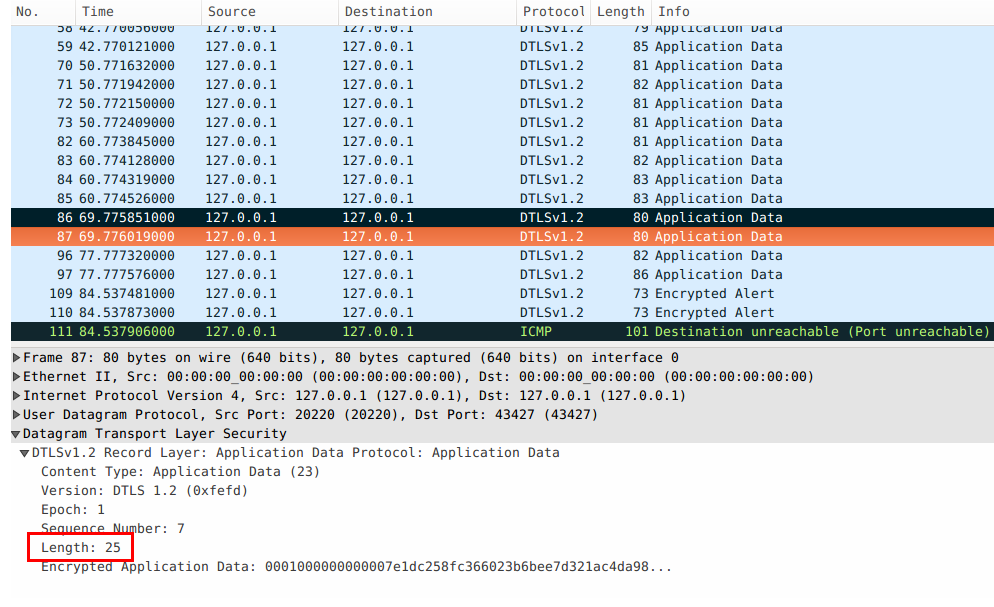
\includegraphics{./Pics/Wireshark01.png}}
\caption{Captured Leaky Coffee packets}
\label{Fig: Captured Leaky Coffee packets}
\end{figure}

\subsection{Session Detection and Segmentation}
The existence of packets implies that a session is taking place between CLIENT and SERVER.

Further more, since there is a significant difference in the timestamp intervals between continuous packets from same session and different session, one can group packets by their timestamps. Typically a threshold of $4$ seconds is good enough for \textbf{Leaky Coffee}. As we can see in the “Time” column in \Cref{Fig: Captured Leaky Coffee packets}\footnote{The in-continuous packet number is a result for filtering DTLS packets on the hosting machine.},
\begin{itemize}
\item Packet $70$ to $73$ is a session with $FlavourRequest$ and $FlavourResponse$.
\item Packet $82$ to $85$ is another session with $FlavourRequest$ and $FlavourResponse$.
\item Packet $86$ and $87$ is a session without $FlavourRequest$ and $FlavourResponse$.
\item Packet $96$ and $97$ is another session without $FlavourRequest$ and $FlavourResponse$.
\item ...
\end{itemize}

Once a session has been segmented, we can immediately label them as described in \Cref{Def: Leaky Coffee Session}.

\subsection{Plaintext Guessing} \label{Sec: Plaintext Guessing}
Similar to \textbf{Odd or Even}(\Cref{Sec: Odd or Even}), ciphertexts exchanged in \textbf{Leaky Coffee} has distinguish length which could possibly be exploited to recover the plaintexts.

To formalise it, we model the leakage through ciphertext lengths as a channel\cite{Information_Theory}, inspired by \cite{Web2}. The general idea is to view the ciphtertext lengths as an input and plaintext the output, then the leakage problem is immediately equivalent  to the decoding problem of such a channel. 

In order to do this, we first construct a  \textbf{Forward Channel} that “encodes” plaintexts to ciphertext lengths. The \textbf{Leakage Channel}, which “decodes” ciphertext lengths to plaintexts, is therefore followed by as the reversion of \textbf{Forward Channel}.

\begin{definition} \label{Def: Channels}
Let $\mathbb{X}$ be the set of possible plaintexts and $\mathbb{Y}$ the set of possible packet lengths in bytes. The \textbf{Forward Channel} is then given as  $\bf{W(y|x)}$ and \textbf{Leakage Channel} as $\bf{W^{-1}(x|y)}$ where both $x \in \mathbb{X}$ and $y \in \mathbb{Y}$.
\end{definition}

\Cref{Ex: Single_Order} describes an example of how Forward Channel and Leakage Channel are constructed.

\begin{example} \label{Ex: Single-Order}
Take $Order$ for example. According to \Cref{Def: Order}, we have:
\begin{equation*}
\mathbb{X} = \{\text{“AMECINANO”}, \text{“CAPPUCINO”}, \text{“MOCHA”}, \text{“ESPRESSO”}\}
\end{equation*}

Hence the Forward Channel is as \Cref{Tbl: Forward Channel for Order}. 
\begin{table}[H]
\begin{center}
{\begin{tabular}{c|l|l|l||l|}
$W(y|x)$          & 5 & 8 & 9 & $P$\\
\hline
"AMERICANO" &   &  & 1  & $1/4$ \\
\hline
"CAPPUCINO" &   &   & 1  & $1/4$\\
\hline
"MOCHA"     & 1 &   &    & $1/4$\\
\hline
"ESPRESSO"  &   &  1  &   & $1/4$\\
\hline
\end{tabular}
}
\end{center}
\caption{Forward Channel for $Order$}
\label{Tbl: Forward Channel for Order}
\end{table}

The ciphertext length is fixed once the plaintext is given; therefore the probability of a ciphertext length could either be $0$ or $1$.

The joint probability immediately follows by:
\begin{equation}
(\widehat{W}P)(x,y) = P(x)W(y|x)
\end{equation}

Which results into \Cref{Tbl: Joint Probability of (X Y) for Order}.

\begin{table}[H]
\begin{center}
{\begin{tabular}{c|c}

$\widehat{W}P$  & P     \\ \hline
("AMERICANO",9) & $1/4$ \\ \hline
("CAPPUCINO",9) & $1/4$ \\ \hline
("MOCHA",5)     & $1/4$ \\ \hline
("ESPRESSO",8)  & $1/4$ \\ \hline
\end{tabular}
}
\end{center}
\caption{Joint Probability of $(\mathbb{X},\mathbb{Y})$ for $Order$}
\label{Tbl: Joint Probability of (X Y) for Order}
\end{table}

Since the events of each $X=x$ are exclusive, the marginal probability of $Y=y$ is the sum of each of its joint probabilities:
\begin{equation}
P(Y=y) = \sum\limits_{x \in \mathbb{X}}{\widehat{W}P(x,y)}
\end{equation}

The result is shown in \Cref{Tbl: Marginal Probabilities of y}.

\begin{table}[H]
\begin{center}
{\begin{tabular}{|c|c|}
\hline
 $y$ & P     \\ \hline
5 & $1/4$ \\ \hline
8 & $1/4$ \\ \hline
9 & $1/2$ \\ \hline
\end{tabular}}
\end{center}
\caption{Marginal probabilities of $y$}
\label{Tbl: Marginal Probabilities of y}
\end{table}

Finally we can construct the Leakage Channel using Bayes’ theorem:
\begin{equation}
P(x|y) = {\frac {P(x)P(y|x)} {P(y)}} 
\end{equation}

And constrcut the Leakage Channel as shown in \Cref{Tbl: Leakage Channel for Order}

\begin{table}[H]
\begin{center}
{\begin{tabular}{c|c|c|c|c|}
$W^{-1}(x|y)$  & “AMERICANO” & “CAPPUCINO” & “ESPRESSO” & “MOCHA” \\ \hline
5 &             &             &            & $1$     \\ \hline
8 &             &             & $1$        &         \\ \hline
9 & $1/2$       & $1/2$       &            &         \\ \hline
\end{tabular}
}
\end{center}
\caption{Leakage Channel for $Order$}
\label{Tbl: Leakage Channel for Order}
\end{table}

The Leakage Channel(\Cref{Tbl: Leakage Channel for Order}) can be then used as a guideline for an eavesdropper adversary to recover the plaintext being transmitted.

\end{example}

One underlining problem in this method is the need to enumerate the plaintext. In some scenarios, it is possible to mitigate this problem by reducing the size of $\mathbb{X}$ by grouping plaintexts. The cost of this mitigation is the loss of resolution in the recovered plaintext, as shown in \Cref{Ex: Single-OrderFlavour}.

\begin{example} \label{Ex: Single-OrderFlavour}
%The first step is to compute the Content-Length channel. Analysis on $Order||Flavour$ packet is more complicated as it has a larger entropy. 
%
%We omit the sequence of SUGAR and MILK to simplify the problem. We also simplify our notation by denoting $D_1$ as the degree of SUGAR and $D_2$ the degree of MILK. Then any $Flavour$ can be represented as $(D_1, D_2)$, e.g. $(2,1)$ represents any $Flavour$ that has a degree of SUGAR 2 and degree of MILK 1.
%
%The same strategy can be applied directly on this example as well. However, the space of this channel is much more complicated in this case which are $4 $
%
%It is sometimes possible to simplify the problem by breaking the Plaintext-Length channel into several sub-channels, namely $Order$ channel $W_{0}(y \in l|x \in COFFEE)$, SUGAR channel $W_{1}(y \in l| x \in D_1)$ and MILK channel $W_{2}(y \in l | x \in D_2)$ in this application. These sub-channels requires less computation and we will show how to reconstruct the Plaintext-Length channel using these sub-channels later in this section. 
%
%Obviously that $W_0$ is identical to \Cref{Tbl: Order1} as the $Order$ part in $Order||Flavour$ is simply an echo of the first $Order$ packet. 
%
%$W_2$ and $W_3$ are actually identical:
%
%\begin{table}[H]
%\begin{center}
%{\begin{tabular}{c|c|c|c|c||l|}
$W_1(x|y)$ & 0 & 1 & 2 & 3 & P     \\ \hline
0          & 1 &   &   &   & $1/4$ \\ \hline
1          &   & 1 &   &   & $1/4$ \\ \hline
2          &   &   & 1 &   & $1/4$ \\ \hline
3          &   &   &   & 1 & $1/4$ \\ \hline
\end{tabular}
}
%{\begin{tabular}{c|c|c|c|c||l|}
$W_2(x|y)$ & 0 & 1 & 2 & 3 & P     \\ \hline
0          & 1 &   &   &   & $1/4$ \\ \hline
1          &   & 1 &   &   & $1/4$ \\ \hline
2          &   &   & 1 &   & $1/4$ \\ \hline
3          &   &   &   & 1 & $1/4$ \\ \hline
\end{tabular}
}
%\end{center}
%\caption{Channels of SUGAR-Length and MILK-Length}
%\label{Tbl: SUGAR-Length and MILK-Length}
%\end{table}
%
%Then we merge $W_1$ and $W_2$ to construct the $Flavour$ - Length channel $W_1 \otimes W_2((y_1, y_2) |(x_1, x_2))$ where $(y_1, y_2) \in l \otimes l, (x_1, x_2) \in D_1 \otimes D_2$:
%
%\begin{table}[H]
%\begin{center}
%{\begin{tabular}{c|c|c|c|c|c|c|c||c|}
$W_1 \otimes W_2((y_1,y_2)|(x_1, x_2))$ & (0,0) & (0,1) & ... & $(y_1, y_2)$             & ... & (3,2) & (3,3) & P         \\ \hline
(0,0)             & 1     &       &     &                          &     &       &       & $1/16$  \\ \hline
(0,1)             &       & 1     &     &                          &     &       &       & $1/16$  \\ \hline
...               &       &       &     &                          &     &       &       &           \\ \hline
$(x_1, x_2)$      &       &       &     & $P((y_1,y_2)|(x_1,x_2))$ &     &       &       & $P(x_1, x_2)$ \\ \hline
...               &       &       &     &                          &     &       &       &           \\ \hline
(3,2)             &       &       &     &                          &     & 1     &       & $1/16$  \\ \hline
(3,3)             &       &       &     &                          &     &       & 1     & $1/16$  \\ \hline
\end{tabular}}
%\end{center}
%\caption{$Flavour$-Length channel}
%\label{Tbl: Flavour channel}
%\end{table}
%
%The right end column of probability is simply the joint probability of both inputs of $W_1$ and $W_2$. 
%
%In this application, degree of SUGAR and degree of MILK are independent variables. This implies their joint probability is simply the product of their marginal probabilities:
%\begin{equation}
%P(x_1, x_2) = P(x_1) P(x_2)
%\end{equation}
%
%Notice that since the output of such channel are actually the length of its input; therefore for a given input, its output is deterministic, i.e.
%\begin{eqnarray} 
%P((y_1,y_2)|(x_1,x_2)) =
%	\begin{cases}
%	1 &\text{if } y_1 = |x_1| \text{ and } y_2 = |x_2| \\
%	0 &\text{otherwise}
%	\end{cases}
%\label{Eq: Length Probability}
%\end{eqnarray}
%
%The merged channel $W_1 \otimes W_2$ results in a table with size of $(|X_1||X_2|)$ rows and $(|Y_1| |Y_2|)$ columns. This implies that the merge operation of two channels will potentially has an exponential time and space complexity. However, this can be improved by compressing the channel.
%
%The first thing is that the merged output are actually lengths of both inputs; hence $(y_1, y_2)$ can be replaced by their sum: $y = y_1 + y_2$. Therefore \Cref{Tbl: Flavour channel} can be compressed by combing columns with a same length, i.e. we can merge columns into one if $(y_1 + y_2) = (y\prime_1 + y\prime_2)$. The combination is simply the vector sum of two columns
%
%So we can reconstruct $W_1 \otimes W_2$ as:
%\begin{table}[H]
%\begin{center}
%{\begin{tabular}{c|c|c|c|c|c|c|c||c|}
$(W_1 \otimes W_2)\prime( y =y_1 + y_2 | (x_1, x_2))$ & 0 & 1 & 2 & 3 & 4 & 5 & 6 & P      \\ \hline
(0,0)             & 1 &   &   &   &   &   &   & $1/16$ \\ \hline
(0,1)             &   & 1 &   &   &   &   &   & $1/16$ \\ \hline
...               &   &   &   &   &   &   &   &        \\ \hline
(1,0)             &  & 1 &   &   &   &   &   &        \\ \hline
...               &   &   &   &   &   &   &   &        \\ \hline
(3,2)             &   &   &   &   &   & 1 &   & $1/16$ \\ \hline
(3,3)             &   &   &   &   &   &   & 1 & $1/16$ \\ \hline
\end{tabular}}
%\end{center}
%\caption{Compressed $Flavour$-Length channel}
%\label{Tbl: Compressed Flavour}
%\end{table}
%
%In \Cref{Tbl: Compressed Flavour}, we can see that different inputs can map to the same length, e.g. $(0,1)$ and $(1,0)$ all results to $l = 1$.
%
%Practically, we can further compress this channel with the cost of resolution of input. Generally, there are some facts that worth notice:
%\begin{itemize}
%\item As in \eqref{Eq: Length Probability},  length is deterministic given a content. Therefore it is a reasonable choice to merge contents which will result into same length.
%\item The intuition of combing two rows with the same length can be interpreted as follow: for two rows with the same output $W(y| x=x_1)$ and $W(y|x=x_2)$, the merged row represents $W(y|x=x_1 \text{ or } x = x_2 )$.
%\item For such a channel, each input are exclusive events; thus the probability of the input of merged rows is simply the sum of the probability of each row: $P(x_{merged}) = P(x_1) + P(x_2)$
%\end{itemize} 
%
%So if we compress \Cref{Tbl: Compressed Flavour} by the same $(y_1 + y_2)$ which is indeed $|Flavour|$, we will have a further compressed $W_1 \otimes W_2$:
%
%\begin{table}[H]
%\begin{center}
%{\begin{tabular}{c|c|c|c|c|c|c|c||c|}
$(W_1 \otimes W_2)''(y = y_1+y_2 | x = x_1 + x_2)$ & 0 & 1 & 2 & 3 & 4 & 5 & 6 & P      \\ \hline
0                     & 1 &   &   &   &   &   &   & $1/16$ \\ \hline
1                     &   & 1 &   &   &   &   &   & $1/8$  \\ \hline
2                     &   &   & 1 &   &   &   &   & $3/16$ \\ \hline
3                     &   &   &   & 1 &   &   &   & $1/4$  \\ \hline
4                     &   &   &   &   & 1 &   &   & $3/16$ \\ \hline
5                     &   &   &   &   &   & 1 &   & $1/8$  \\ \hline
6                     &   &   &   &   &   &   & 1 & $1/16$ \\ \hline
\end{tabular}
}
%\end{center}
%\caption{Further Compressed (with less resolution) $Flavour$-Length channel }
%\label{Tbl: Further Compressed Flavour}
%\end{table}
%
%The actual degree of SUGAR and MILK are lost in \Cref{Tbl: Further Compressed Flavour} during this compression, but it also reduced the number of rows from $16$\footnote{$(W_1 \otimes W_2)\prime$ has $4 \times 4 = 16$ rows.} to $7$.
%
%By applying the same strategy again to merge the $Order$ channel $W_0$ with $(W_1 \otimes W_2)$, we will have the $OrderFlavour$-Length channel $W = W_0 \otimes W_1 \otimes W_2$. Then finally as described in \Cref{Exmp: Single-Order}, we can construct the leakage channel $W^{-1}(x|y)$ (see \Cref{OrderFlavour leakage channel}) for the $OrderFlavour$ packets .
\end{example}
%
%To generalise, given the distribution of the plaintext, the leakage channel is constructed as following:
%\begin{description}
%\item[1] If the space of plaintext is large, break the plaintext-length channel into several sub-channels.
%\item[2] Compute the sub-channels and compress them. Resolution may lost during the compression.
%\item[3] Merge the sub-channels to construct the plaintext-length channel.
%\item[4] Use Bayes’ Theorem to invert plaintext-length channel.
%\end{description}
%
%Another aspect to view such leakage channel is to analyse its capacity, i.e. the maximum mutual information of content and length, as described in \cite{Web2}.
%
%\subsection{Guessing Plaintext Using Joint Packet Length} \label{Sec: Guessing Plaintext Using Joint Packet Length}
% In \Cref{Sec: Guessing Plaintext by One Packet Length} we described a method of packet analysis against a single packet in a session. It is possible to improve the analysis by looking at the packets jointly. As presented in \cite{Web2}, the sequence of packets lengths can be viewed as a vector.



%For example, a 2-packets session (packet No 86 and 87) has been marked out in \Cref{Fig: Captured Packets 01}. The values of DTLS Length  are both $25$ as marked in red rectangle. Their actual plaintext length can then be computed as $8$ and $8$ bytes respectively by \Cref{Eq: Plaintext length}. 
%
%It is possible to do the single packet analysis described in \Cref{Sec: Guessing Plaintext by One Packet Length} on each of these packets. We immediately know that plaintext in the first packet is “ESPRESSO”; whilst the second one could be either “ESPRESSO” or “MOCHA” with a $Flavour$ of length $3$. However, the analysis of the second packet is in fact unnecessary at all as the application specifies that an “ESPRESSO” $Order$ can only be responded with an “ESPRESSO” with NULL $Flavour$.
%
%The application specifies that the first part of the $Order||Flavour$ simply echoes the first packet; therefore in fact we can immediately tell that the second packet is “ESPRESSO”.
%\end{example}
%
%One way to model this is to “expand” the channel. Instead of using the content at each packet from as the input, we can write them as a vector:
%\begin{equation*}
%\vec{x} = <x_1, x_2, ..., x_n>
%\end{equation*}
%
%and similarly, we can also write their length as another vector:
%\begin{equation*}
%\vec{l} = <y_1, y_2, ..., y_n>
%\end{equation*}
%
%Then we can use the same strategy in \Cref{Sec: Guessing Plaintext by One Packet Length} to construct the leakage channel $W^{-1}(X, Y)$ where $\vec{x} \in X$ and $\vec{y} \in Y$. 
%
%A problem in this method is the resulting channel is of the size of the Cartesian product of all contents in every packet. However, in this Leaky Coffee application most of the cells is actually $0$ which could be used to reduce its storage space; but such optimisation is heavily application dependant.
%
%A probably better way to model this side channel is to use Hidden Markov Model\cite{baum1966} similar to \cite{Danezis_trafficanalysis}. Techniques of Machine Learning might also be able to utilise this side channel information more efficiently. However, in this “intentionally crafted” Leaky Coffee application, the first packet seems always enough to reveal (roughly) the rest of plaintext in a session.
%
%\subsection{Estimate plaintext distribution}
%In \Cref{Sec: Guessing Plaintext by One Packet Length} and \Cref{Sec: Guessing Plaintext Using Joint Packet Length} we have demonstrated how to construct a channel given the set of plaintext and their distribution. In this section, we will try to estimate the plaintext distribution by the distribution of ciphertext.
%
%The general idea is that the distribution of length (as presented as $P$ column in \Cref{Tbl: Order3}) can actually be observed from the ciphertext; therefore we can revert the process and use it to estimate the distribution of plaintext.
%
%\begin{example}
%Assume we have a sample of encrypted $Order$ packet collected where we estimated the its length distribution as following: 
%\begin{table}[H]
%\begin{center}
%{\begin{tabular}{|c|c|}
\hline
 $y$ & P     \\ \hline
5 & $d_1$ \\ \hline
8 & $d_2$ \\ \hline
9 & $d_3$ \\ \hline
\end{tabular}
}
%\end{center}
%\caption{Estimated length distribution from encrypted $Order$ packets}
%\label{Tbl: Estimated length distribution from encrypted $Order$ packets}
%\end{table}
%
%Similar to \Cref{Exmp: Single-Order}, the first step is to construct a Content-Length channel. The difference is that this time we do not have the pre-knowledge of plaintext distribution; therefore we represent the content distribution as unknown variables $p_i$ for each content.
%
%\begin{table}[H]
%\begin{center}
%{\begin{tabular}{c|l|l|l||l|}
$W(y|x)$          & 5 & 8 & 9 & $P$\\
\hline
"AMERICANO" &   &  & 1  & $p_1$ \\
\hline
"CAPPUCINO" &   &   & 1  & $p_2$\\
\hline
"MOCHA"     & 1 &   &    & $p_3$\\
\hline
"ESPRESSO"  &   &  1  &   & $p_4$\\
\hline
\end{tabular}
}
%\end{center}
%\caption{Content-Length Channel with unknown distibution of $Order$}
%\label{Tbl: Content-Length Channel with unknown distibution of $Order$}
%\end{table}
%
%
%%Since we are only interested in $p_1$ and $p_3$ and the appearance of each content is exclusive, \Cref{Tbl: Content-Length Channel with unknown distibution of $Order$} can be rewritten as \Cref{Tbl: Rewritten Content-Length Channel with unknown distibution of $Order$}.
%%
%%\begin{table}[H]
%%\begin{center}
%%{\begin{tabular}{c|c|c|c||c|}
$W(y|x)$          & 5 & 8 & 9 & $P$\\
\hline
"AMERICANO" &   &  & 1  & $p_1$ \\
\hline
"MOCHA"     & 1 &   &    & $p_3$\\
\hline
"ESPRESSO" or "CAPPUCINO"  &   &  $p_4 / (p_2 + p_4)$  &  $p_2 / (p_2 + p_4)$  & $p_4 + p_2$\\
\hline
\end{tabular}
}
%%\end{center}
%%\caption{Rewritten Content-Length Channel with unknown distibution of $Order$}
%%\label{Tbl: Rewritten Content-Length Channel with unknown distibution of $Order$}
%%\end{table}
%
%Their joint distribution follows immediately.
%
%\begin{table}[H]
%\begin{center}
%{\begin{tabular}{c|c}

$\widehat{W}P$  & P     \\ \hline
("AMERICANO",9) & $p_1$ \\ \hline
("CAPPUCINO",9) & $p_2$ \\ \hline
("MOCHA",5)     & $p_3$ \\ \hline
("ESPRESSO",8)  & $p_4$ \\ \hline
\end{tabular}
}
%\end{center}
%\caption{Joint distribution of $(Order, l)$ with unknown distribution of $Order$}
%\label{Tbl: Joint distribution of $(Order, l)$ with unknown distribution of $Order$}
%\end{table}
%
%Then we can compute the marginal distribution of length.
%
%\begin{table}[H]
%\begin{center}
%{\begin{tabular}{|c|c|}
\hline
 $y$ & P     \\ \hline
5 & $p_3$ \\ \hline
8 & $p_4$ \\ \hline
9 & $p_1 + p_2$ \\ \hline
\end{tabular}}
%\end{center}
%\caption{Marginal distribution of $l$ with unknown distribution of $Order$}
%\label{Tbl: Marginal distribution of $l$ with unknown distribution of $Order$}
%\end{table}
%
%By linking \Cref{Tbl: Marginal distribution of $l$ with unknown distribution of $Order$} with \Cref{Tbl: Estimated length distribution from encrypted $Order$ packets} we have the following constrains to the content distribution:
%
%\begin{equation} \label{Eq: Plaintext Distribution Estimation}
%\left \{
%\begin{aligned}
%p_3 = d_1\\
%p_4 = d_2\\
%p_1 + p_2 = d_3\\
%\sum\limits_{i = 1}^4{p_i} = 1
%\end{aligned}
%\right
%\end{equation}
%
%Any solution satisfies \Cref{Eq: Plaintext Distribution Estimation} can be viewed as a reasonable guess to the distribution of the contents.
%
%\end{example}
